\clearpage
\section{Neuroevolution}

In this section we discuss \textit{neuroevolution}, a subtype of genetic algorithm that is specifically designed to train neural networks. After a brief overview of some of the key concepts, we describe how we used the technique in our game to train the behaviour of the enemy frog.

\subsection{Overview}

The key idea behind neuroevolution is to treat neural networks as the chromosomes in a genetic algorithm. The weights of the connections between neurons (and potentially the connections themselves) are treated as genes. Neuroevolution is particularly suited to problems where labelled training data does not exist but where it \textit{is} possible to compare the quality of solutions via a fitness function. The lack of labelled training data makes it impossible to train a network using backpropagation, but evolutionary methods still work because they do not care what the networks calculate; they only care about the effectiveness of each solution.

\begin{figure}[!htbp]
    \centering
    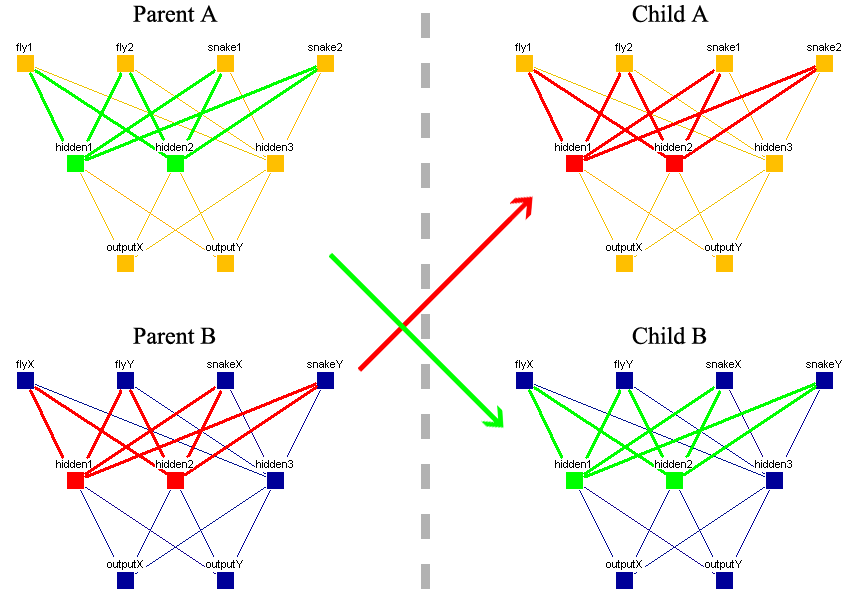
\includegraphics[scale=0.6]{Figs/Crossover.png}
    \caption{A crossover operation applied to neural networks. Here, there are two genes crossed over.}
    \label{fig:netCrossover}
\end{figure}

In neuroevolution, the crossover operation generally yields stronger children when input weights to the same neuron are treated as a single gene. This is because such weights may be finely tuned in relation to each other, so cutting halfway between them may ruin the neuron's precise configuration. Figure \ref{fig:netCrossover} illustrates the preferred type of crossover. While there are eight connection weights involved, this corresponds to only \textit{two} genes being swapped. Mutation, on the other hand, still perturbs weights individually.

\subsection{Neuroevolution in Our Game}
Automating the behaviour of the enemy frog in our game struck us as a potentially interesting application for neuroevolution. Our goal was to train a neural network that, given a set of real-time game data (such as the relative positions of the nearest flies, snakes, obstacles and lakes), would output an appropriate $(x, y)$ steering for the frog. Of course, we could have hardcoded a list of behavioural options for the frog and had the neural net choose between plans, or we could have taught the frog how to behave based on data recorded from human play, but we wanted the frog to learn by itself from scratch!

\subsubsection{Network Architecture}
\noindent We designed the input layer of the neural networks to be dynamic so that the number of flies, snakes, obstacles and lakes fed in could be changed easily from the inspector in Unity. This setup allowed us to experiment with training simple tasks first (e.g. catching stationary flies with no predators or obstacles) then increase the difficulty as we discovered what the frogs were capable/incapable of learning. In the final configuration we used to train the in-game frog, the network was supplied with the nearest two flies, snakes and obstacles, and the nearest lake. Each object requires two inputs ($x$ and $y$), so this gave a total of 14 inputs. We also fed in the frog's current water level so that the frog could theoretically learn to approach snakes when it had enough water to fire a bubble and return to the lake when its water level got low. (More on this in Section \ref{sec:bubbles}).

The input vectors were calculated relative to the frog; i.e. the vector from the frog to each object was used, not the object's world co-ordinates. In the literature we saw that it is common to also normalise angles to the agent's co-ordinate system, but we experimented with this approach and found that it was not of much help. The problem with normalising angles is that the frog's rotation does not particularly matter in our game. The frog's turn speed is so fast that it does not matter if, for example, the frog is facing a snake or has its back turned (see Figure \ref{fig:NormalisationProblem}). If angles are normalised then these scenarios are presented as different inputs, even though the frog's behaviour should probably be the same either way.

\begin{figure}[!htbp]
    \centering
    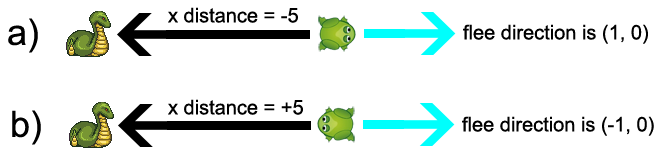
\includegraphics[scale=0.6]{Figs/NormalisationProblem.png}
    \caption{In the frog's co-ordinate system, these scenarios are different and require different responses. The frog has to learn different behaviours for every orientation it is in. World co-ordinates are no better, since the frog must learn different behaviours for every rotation of the vector to the snake.}
    \label{fig:NormalisationProblem}
\end{figure}

Our solution to this problem was somewhat crude, but it makes full use of the rotational symmetry of the game. The inputs are fed into the network \textit{multiple} times, with a different rotational transform applied to the input vectors at each iteration (from $0\degree$ to $360\degree$). The reverse transformation is then applied to the output, and the average is taken across all iterations. This makes the frog's behaviour completely invariant to rotations.\footnote{Technically this is only approximate, but as long as the increments are fine enough then the frog's behaviour will be very close to rotation-invariant. There is probably a clever mathematical way of ensuring that a neural network is invariant to rotations, but we are not aware of such a method.} We found that this approach drastically increased the frogs' learning rate.

A final note regarding input transformations is that it does not really make sense to feed in the differential from the frog to each game object directly. This would mean that the farther away a game object became, the larger an input signal it would send. Even worse, a snake that was just about to bite the frog would send only a tiny signal! For this reason, we rescaled the magnitude for each input vector according to Equation \ref{eqn:1}:

\begin{align}
\text{\textit{Input magnitude}} = e^{-k\|V\|}
\label{eqn:1}
\end{align}

where $V$ is the vector from the frog to the object and $k$ is a dampening constant (equal to 10 in our implementation for all object types).

For the hidden neurons, we chose to use a single layer for simplicity. Generally speaking, the more complex the architecture, the longer the network takes to train. The textbook\footnote{\textit{AI Techniques For Game Programming}} example we followed only had four inputs, so we were already worried that our architecture was too complicated! Likewise, the \textit{NEAT} algorithm that we saw in class was very interesting, but we did not think we had enough time to experiment with evolving the network architecture. The number of neurons in our hidden layer was configurable, but we used 7 in our final training run.

Importantly, the squashing function had to be an odd function (in the mathematical sense) to preserve the symmetry between the positive and negative axes of the game world. We chose to use a logistic curve, scaled to the range (-1, 1). Similarly, it would not make sense to use a bias (i.e. to shift the logistic curve left or right) since that would also break the spatial symmetry. Instead, we evolved the co-efficient of the exponent in the logistic function (i.e. we evolved $k$ in $1/(1 + e^{-kt})$) so that the frogs could still learn an appropriate compression for the input signals.

As we already mentioned earlier, the output of our neural net was the $(x, y)$ steering of the frog. The only tweak we had to make was to multiply the output by a constant so that the speed of the frog was sensible.

\subsubsection{Fitness function}

Our fitness function went through several iterations, but the final one we used was:

\begin{align}
\textit{\text{fitness}} = \textit{\text{(flies caught)}} - 7.5 * \textit{\text{(damage taken)}} - 0.5 * \textit{\text{Min}(0, }\textit{\text{5 - (water camping score)}}\textit{)}
\label{eqn:2}
\end{align}

where the ``water camping score'' increments by 1 for every second a frog spends in a lake when it already has full water. The \textit{Min} function serves as a grace period so that the frogs can accumulate a water camping score of 5 before they actually start to be penalised. For the subsequent parent selection, we used ranked roulette.

\subsubsection{Challenges}

In this section we discuss some of the challenges we faced while training the frogs and the steps that we took to overcome them.

\subsubsection{Smart, Yet Undesirable Behaviour}

A major problem we encountered was that the frogs often evolved towards a high fitness solution, but the corresponding behaviour was not what we wanted or expected. Some examples are provided below:\\

\hspace*{-0.27in}
\begin{tabular}
{|p{10.7cm}|p{6.8cm}|}
\hline
\textbf{Problem} & \textbf{Solution}\\
\hline
If the training pens contained a large number of flies that were configured to wander around the pens, the frogs learned to avoid the snakes, but not to target the flies. This is because the frogs were likely to catch many flies by pure chance. The frogs that were slightly biased to target the flies tended to get hit slightly more often too, which cancelled out their advantage. They may have learned to target the flies eventually but it was not apparent in our experiments. If there were too few flies then funnily enough the same thing happened, since there was not enough positive reinforcement for the frogs when they caught flies. & We made the flies stationary during training so that the frogs that deliberately targeted them got more of an advantage. We used trial-and-error to finely tune the number of flies in each training pen. We also tuned the reward size for catching a fly relative to the punishment for being hit by a snake. In retrospect, it may have been useful to decrease this ratio as training progressed.\\
\hline
Since the punishment for being hit by a snake was much larger than the reward for catching a fly, the frogs naturally learned to protect themselves first and foremost. Unfortunately, the most effective defense was to run into a lake and stay there! Once the entire population learned this behaviour, training stagnated because the frogs never left the lake and had little opportunity to learn about the reward for catching flies. & We introduced a ``water camping'' penalty to the fitness function, as mentioned above in Equation \ref{eqn:2}. Admittedly this was ``cheating'' -- ideally the frogs would have learned to leave the lake by themselves -- but the cheat was very effective!\\
\hline
The training runs were originally fairly short (20 seconds long), but this lead to overly-aggressive behaviour. The frogs that focused on catching flies and completely disregarded the snakes tended to rank first every time, because the snakes were configured to wander, and chances were that several frogs would receive favourable runs where the snakes wandered away from the largest fly clusters. & We increased the time limit to 2 minutes per training run in order to expose over-aggression. We also configured the fly distribution to be the same across pens. The distribution was still randomised at the start of each epoch, but stored in a static variable shared between pens.\\
\hline
\end{tabular}

\subsubsection{Training Time}
As mentioned in the last problem above, the training runs needed to be reasonably long in order to expose poor behaviours. However, we found that it generally took around 1,500 epochs for the frogs' learning to become saturated (see later, Figure \ref{fig:FrogFitness}). A typical population size in these type of GA experiments is 30 -- 50, which would have meant an epoch time of over an hour had we not found some efficiency gains! Our first measure was to increase the Unity time scale. We found that a factor of 4 worked without making Unity unstable. Our second measure was to duplicate the training pens (see Figure \ref{fig:TrainingPens}). With eight indentical pens, a population size of 40 only required 5 batches of frogs per epoch. We could have created even more pens, but Unity was taking a long time to launch the scene with so many resources loaded at once.

\begin{figure}[!htbp]
    \centering
    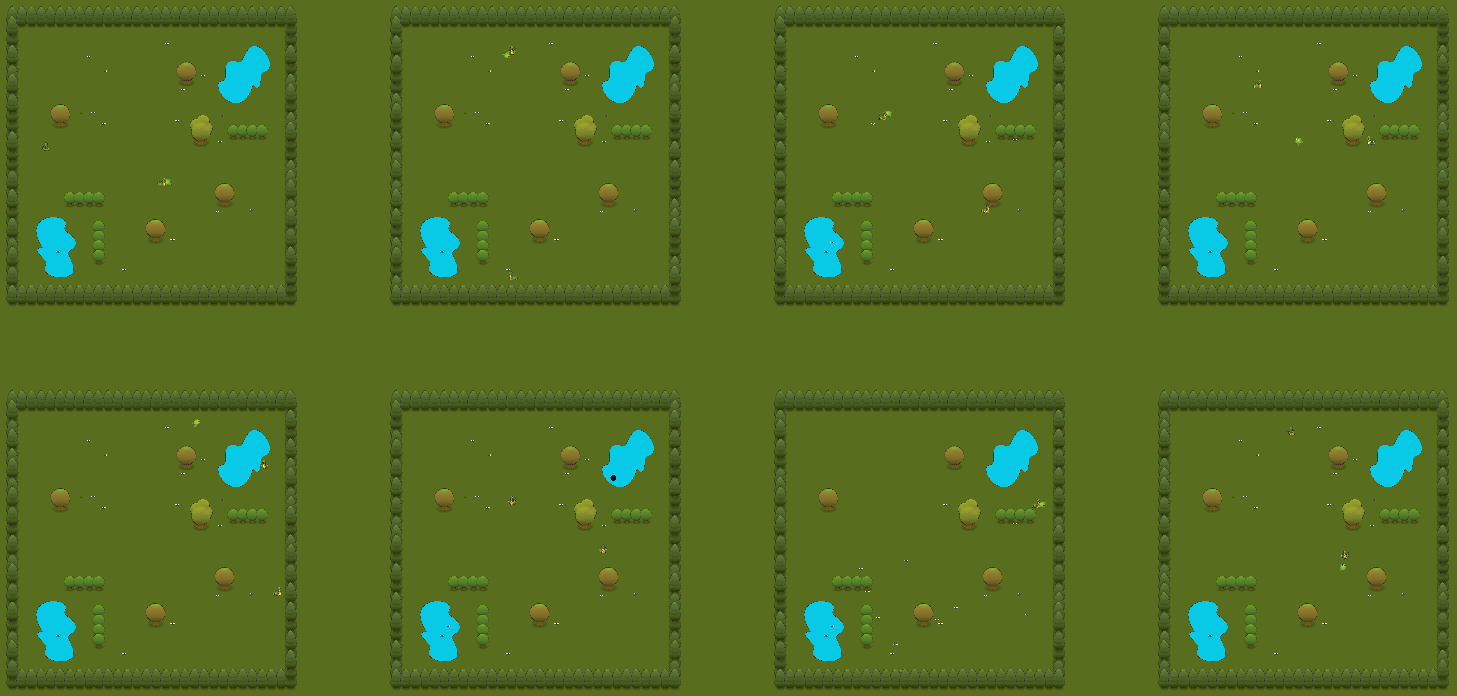
\includegraphics[scale=0.3]{Figs/TrainingPens.png}
    \caption{The training pens we set up to train several frogs simulataneously.}
    \label{fig:TrainingPens}
\end{figure}

\subsubsection{Obstacle Avoidance}
In the original game, the frog was controlled by mouse clicks and avoided obstacles via a combination of A* and a few tricks to avoid corner collisions. This time the frog was controlled by a neural network, which was essentially just another type of steering behaviour. This created a problem, because A* and steering behaviours do not really gel. A* requires a goal node, but steering behaviours only provide a direction of travel, not a distance. Our solution was to modify the obstacle avoidance technique that the flies used in our first assignment so that the frogs could use it as well. This meant that the frog was no longer capable of navigating mazes, so we had to ensure that the maps we used for training and the actual game did not include any ``bowl'' shapes that would trap the frog.

\subsubsection{Shooting Bubbles}
\label{sec:bubbles}
We wanted the frog to learn to shoot bubbles after filling up on water in the lakes, but we decided that having the frog learn this behaviour from scratch would be too difficult, especially given our time limits. Opportunities to fire on snakes are limited, and the overall plan of \textit{obtain water} $\rightarrow$ \textit{approach snake} $\rightarrow$ \textit{fire at correct angle} is quite a complex one, particularly since the frogs must learn to avoid the snakes in general. Our solution was to script the frog to fire directly at snakes within a certain range when the water level is sufficient. We added an additional gene for the frogs' shot range, so the frogs learned \textit{when} to shoot, but not \textit{how} to shoot.

Since bubbled snakes present far less danger to the frog, we needed some way of encoding this into the network input. We considering adding new input neurons for bubbled snakes, but this seemed wasteful given that the inputs would be sending a zero signal the majority of the time, and inaccurate in a sense because the frog would be unaware of how much bubble time the snakes had left (without adding a further input). Our solution was to still represent the bubbled snakes as ordinary snakes, but to increase their distance from the frog (in the input encoding) based on how much bubble time they had left. This way, it seems to the frog as if the bubbles push the snakes backwards, then the snakes run back to their bubbled position as the timer runs out.

\subsection{Outcome}
As we alluded to in the \textit{Challenges} section, we found that the frogs generally learned tasks in a particular order. Since the fitness lost from being hit by a snake far outweighed the benefit from catching a fly, the frogs always learned to protect themselves first. Before we added lakes to the training pens, this meant that the frogs learned to flee from snakes in the opposite direction. After we added lakes, the frogs learned to dive into a lake at the start of every training run. Gradually however, the frogs that had a tendency to catch more flies (and to stay out of the lake, after we added the ``water camping'' penalty) became more and more dominant. Eventually the frogs' behaviour became more daring when flies were positioned close to snakes, and their flee steering became more elaborate and ``slippery''.

Given that the frogs learned completely from scratch (besides some rather involved cheating for the water bubbles), we were very happy with their overall performance. They clearly became stronger throughout training from a qualitative standpoint, but we were also able to confirm that the genetic algorithm worked in a scientific sense by plotting the average population fitness versus epoch from our final training run:\\

\begin{figure}[!htbp]
    \centering
    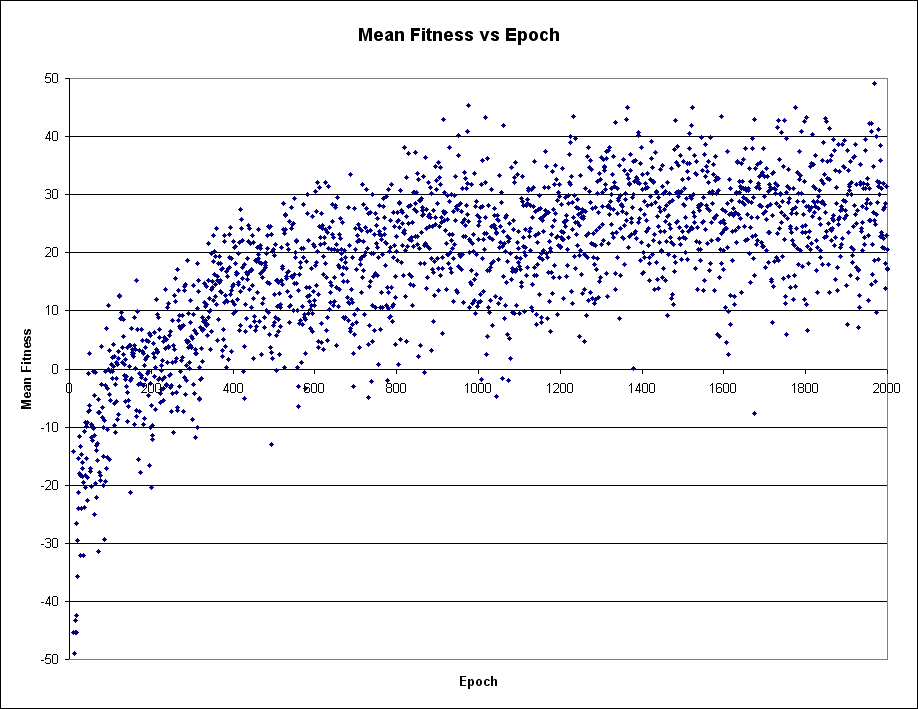
\includegraphics[scale=0.55]{Figs/FrogFitness.png}
    \caption{The total population fitness of the frogs versus the epoch count over 2000 epochs. The training time per epoch was 2 minutes.}
    \label{fig:FrogFitness}
\end{figure}

There is a lot of variance in Figure \ref{fig:FrogFitness} due to the fly spawn locations changing every epoch, but there is a noticeable trend upwards in performance until around epoch 1,500. At that point the population fitness reaches an average of around 25, which corresponds to each frog catching 25 flies without being hurt, and an additional 7.5 flies for each unit of damage taken.